\documentclass{article}
\DeclareMathSizes{10}{10}{7}{7}
\usepackage{amsmath}
\usepackage{ amssymb }
\usepackage{tikz, graphicx}
\usepackage{geometry}
\usepackage[makeroom]{cancel}
\usepackage[export]{adjustbox}
\usepackage[backend=biber]{biblatex}
\usepackage{natbib}
\DeclareMathOperator{\sech}{sech}
\usepackage{subfig}
\usepackage{hyperref}
\hypersetup{
    colorlinks=true,
    linkcolor=blue,
    filecolor=magenta,      
    urlcolor=blue,
    }
\usepackage{float}
\restylefloat{table}

\geometry{legalpaper, margin=0.7in}

\title{Noize net | WORK IN PROGRESS}
\author{Liam Watson}
\begin{document}
\maketitle
\section{Abstract}
Complete abstract at the end
\section{Intorduction to Neural networks}
\label{sec:intro}
Before we procede to the more advanced recurant neural network let us begin with an abbrevated coveradge of neaural networks and the convepts underpining them. 
\subsection{Perceptrons}
\label{sec:peceptrons}
The simplest unit of a neural network is, as the name suggests a neuron or more commonly a peceptron. In it's simplest form a peceptron recieves an input, performs some calculation and produces output.
\begin{figure}[h]
\caption{Peceptron showing N input variables, N weights and a bias}
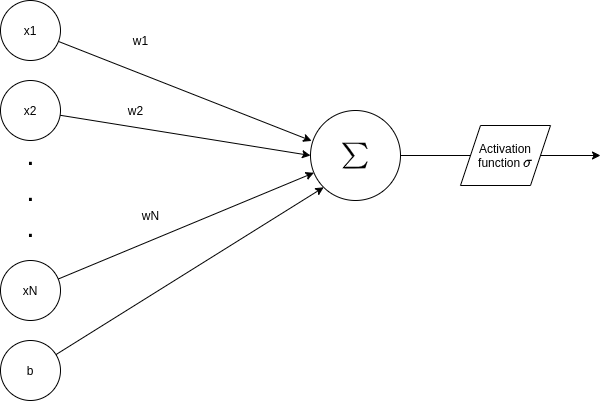
\includegraphics[scale=0.5]{peceptron.png}
\end{figure}
Given these inputs and bias we can adjust weights and bais to satisfy our desired output after summation and activation function (\ref{sec:activationfuncs}). 
More rigorously: Given some input $\{x_i\} \forall i\in \mathbb{Z^+}$ predict some $y=\sigma(W_i x_i)$ where $\sigma$ is some activation function. NOTE PECEPTRON VS ARTIFICIAL NEURON
\subsection{Multi layer peceptrons}
\label{sec:mlp}
Peceptrons, however, are not powerful in this form, rather we only begin to see the utility when we start connecting them together in a mesh much like neurons in the brain. In figure two we can see a depiction of this with weights represented as line thickness (\autoref{fig:mlp}).
\begin{figure}[h]
\caption{Image of a simple neural network archutecture with 8 inputs two hidden layers and four output neurons}
\label{fig:mlp}
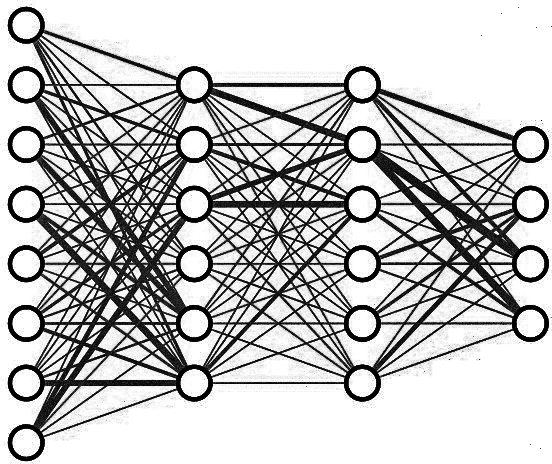
\includegraphics[scale=2]{nn.jpg}
\href{https://www.youtube.com/watch?v=aircAruvnKk&ab_channel=3Blue1Brown}{Sorce}
\end{figure}
\subsection{Gradient decent}
Now we need a way to determine the peceptron weights, for this we use Gradient decent. There are many adaptions of gardient descent that aim to optimize its computational performance or over come some issue with converging to a poory optimised solution such as Fast gradient methods or momentum adapted gradient descent. \\
The aim of gradient descent is to itteratively optimize the peceptron weights to converge on a local minimum by taking steps in the direction of steepest descent, after many itterations we will find that the networks weights are well optimised for some goal. However we may find that a local minimum is not sufficient for our purposes and as such may need to employ some hyperparameter tuning such as changing the the step size we take or adding momentum in the hopes that we converge to a more optimal solution.
\label{sec:gradientDecent}
\begin{figure}[H]
\caption{A plot of $f(x,y) = \sin(x) + \sin(y)$ with a path showing gradient decent steps}
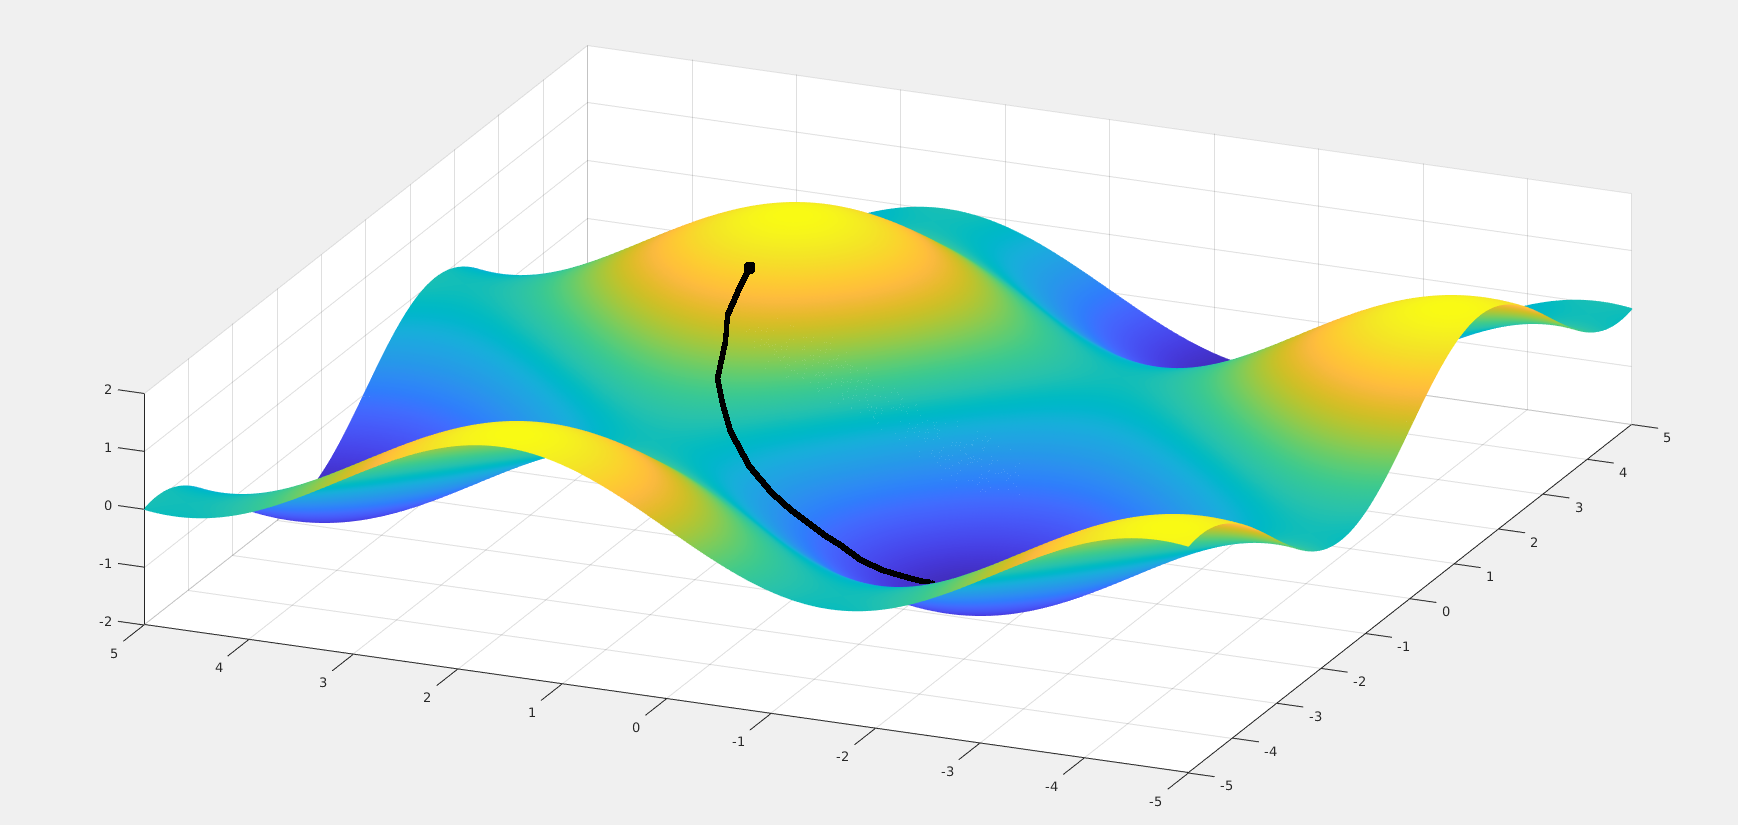
\includegraphics[scale=0.2]{mesh.png}
\end{figure}
\subsection{Activation functions}
Now we will discuss, much like with a biological neuron, how will a neuron decide to acivate or not. There are many functions that are used in the literature but here we give give a quick overview of the most common functions and their uses. The purpose of an activation function is to format the output of a peceptron, we begin with the most elementary of these functions (excluding the identity function defined as $f(x) = x$. 
\begin{enumerate}
\item The binary step function 
Definition:
\begin{align*}
f(x) = 
\begin{cases}
 1 & \text{if } x > 0 \\
 0 & \text{if } x \leq 0 \\
\end{cases}
\end{align*}
The binary step function is primarly used for true, falue classification where the result is not a probability but a certanty. Beyond this this activation function has limited use in modern neural networks, hoever it should be noted that it is very computationally efficient. 
\item Rectified Linear Unit(ReLU)
Definition: 
\begin{align*}
f(x) =
\begin{cases}
 0 & \text{if } x \leq 0 \\
 x & \text{if } x > 0 \\
\end{cases}
\end{align*}
The ReLU Function finds much use dispite its simplicity mostly due to its computational efficiency when compared to the more complex activation functions. ReLU reduces the input domain to only non-negative numbers which can be useful in cases where one wishes to disregard such values. 
\item Sigmoid
Definition: 
\begin{align*}
f(x) =
\begin{cases}
 0 & \text{if } x \leq 0 \\
 x & \text{if } x > 0 \\
\end{cases}
\end{align*}
\item Softmax
Definition: CHANGE THIS
\begin{align*}
f(x) =
\begin{cases}
 0 & \text{if } x \leq 0 \\
 x & \text{if } x > 0 \\
\end{cases}
\end{align*}

\end{enumerate}

\label{sec:activationfuncs}

\subsection{Feed forward}
\label{sec:forward}
NB: NEED TO WRITE MUCH MORE HERE
During the feed forward stage of a network we will recieve input's at the input neurons and travel through all the network layer calculating sum's and activations until the algorithm reaches the output layer.
\subsection{Error functions}
\label{sec:error}
Once we have output from the model, we need a metric for the error between the output and ground truth, an error function. There are many error functions that appear in the litterature, however, their use is often highly application dependent. In the case of Noize net we are dealing with simple two dimensional time series data and as such the relevant error functions are elementary:
\begin{enumerate}
\item Mean Square Error (MSE)\\
This error function finds the averadge square difference between the predicted value and ground truth, defined as
\begin{align*}
MSE = \frac{\sum_{i=0}^N (y_i - y_i^\prime)^2}{N}
\end{align*}
Where $N$ is the number of output values, $y_i$ is the ground truth value and $y_i^\prime$ is the predicted value. \\
This loss function is favorable because of it's simplicity and computational efficiency. One should note that MSE can "amplify" large errors and squah small errors due to the square and notice that the direction of the error is also ignored.  
\item Mean absolute error \\
If one would not like to square the error in order to better capture small errors one can use the MAE function which shares many similar properties with the MSE function but more accurately depicts the difference between a prediction and the ground truth. 
\begin{align*}
MAE = \frac{\sum_{i=0}^N |y_i - y_i^\prime|}{N}
\end{align*}
\item Mean Bias error \\
If the appliction requires a signed error function the MBE error function could be applicable. However, one should note that possitive and negative values may cancel each other out leading to unpredicatble results in practice. 
\begin{align*}
MBE = \frac{\sum_{i=0}^N (y_i - y_i^\prime)}{N}
\end{align*}
\end{enumerate}
\subsection{Back propigation}
\label{sec:back}
Back propigation is the learning step for a model. Once we have completed the feed forward step and calculated the error we need to travel back through the network and adjust the weights and biases in order to optimize the model. FOr this we will use gradient descent.
NB: We need to add the maths here 

\section{Intorduction to Recurrant Neural Networks}
\label{sec:intoRNNs}
When using neural networks for time series data prediction, some semblance of memory is required for sucsessive predictions. Unfortunately standard multi-layer peceptron and convolutional neural networks tend to lose this information quickly as they train due to the vanashing gradient problem. RNNs seek to resolve this by constructing hand crafted compositions of so called "gates" that can encorperate prior information for sucsessive predictions. 

\subsection{RNN concepts}
\label{sec:RNNS}

\subsection{LSTM}
\label{sec:LSTM}

\section{Noize net}
\label{sec:nn}
\subsection{Data and preprocessing}
The data used for training, validation and prediction is the free music \cite{fma dataset}

\label{sec:data}

\subsection{Architecture}
\label{sec:arch}
\subsection{Implimentation}
\label{sec:impl}
\subsection{Results}
\label{sec:results}
\subsection{Conclusion}
\label{sec:conclusion}

\bibliography{References}
\printbibliography[heading=bibintoc]
\begin{filecontents}{References.bib}
@inproceedings{fma dataset,
  title = {{FMA}: A Dataset for Music Analysis},
  author = {Defferrard, Micha\"el and Benzi, Kirell and Vandergheynst, Pierre and Bresson, Xavier},
  booktitle = {18th International Society for Music Information Retrieval Conference (ISMIR)},
  year = {2017},
  archiveprefix = {arXiv},
  eprint = {1612.01840},
  url = {https://arxiv.org/abs/1612.01840},
}
\end{filecontents}

@inproceedings{fma challenge,
  title = {Learning to Recognize Musical Genre from Audio},
  subtitle = {Challenge Overview},
  author = {Defferrard, Micha\"el and Mohanty, Sharada P. and Carroll, Sean F. and Salath\'e, Marcel},
  booktitle = {The 2018 Web Conference Companion},
  year = {2018},
  publisher = {ACM Press},
  isbn = {9781450356404},
  doi = {10.1145/3184558.3192310},
  archiveprefix = {arXiv},
  eprint = {1803.05337},
  url = {https://arxiv.org/abs/1803.05337},
}
\end{document}